\documentclass[10pt, svgnames, beamer, aspectratio=169]{beamer}


\usetheme{Darmstadt}
\setbeamertemplate{headline}{}
\usepackage{fontawesome}
\def\twitter{{\FA \faTwitter}}
\def\github{{\FA \faGithub}}
\def\mail{{\FA \faEnvelope}}
\usepackage[english]{babel}
\usepackage{graphicx}
\usepackage{aeguill}
\usepackage{ucs}
\usepackage{listings}
\usepackage{alltt}
\usepackage{amsmath}
\usepackage{color}
\usepackage{url}
\usepackage{wasysym}
\usepackage{xcolor}
\usepackage{textcomp}
\usepackage{paracol}
\urlstyle{sf}
\usepackage{eurosym}
\usepackage{tikz}
\usetikzlibrary{positioning}
\usetikzlibrary{calc}
\usetikzlibrary{calc,intersections, positioning, automata, decorations.pathreplacing, calc}
\tikzstyle{every picture}+=[remember picture]
\usepackage{amsmath, amsfonts, wasysym}
\usepackage[scaled=0.9]{beramono}

\usepackage{caption}
\DeclareCaptionFont{white}{\color{white}}
\DeclareCaptionFormat{listing}{\footnotesize{#3}}
\captionsetup[lstlisting]{format=listing}


\beamertemplatenavigationsymbolsempty

%\newcommand{\qb}{\textcolor{qbred}{QUARKS}\textcolor{qbgrey}{LAB}} 

%%%%%%%%%%%%%%%%%%%%%%%%%%%%%%%%%%%%%%%%%%%%%%%%%%%%%%%%%%%%%%%%%%%%
% Code Listings %%%%%%%%%%%%%%%%%%%%%%%%%%%%%%%%%%%%%%%%%%%%%%%%%%%%%%%%%%%%%%%


\newcommand{\simdfourvectorclimpl}[8]{
    \def\N{4}
	\pgfmathparse{\L/2}
	\let\XA\pgfmathresult
	\pgfmathparse{\L/2 + \L}
	\let\XB\pgfmathresult
	\pgfmathparse{\L/2 + 2*\L}
	\let\XC\pgfmathresult
	\pgfmathparse{\L/2 + 3*\L}
	\let\XD\pgfmathresult
    \tikz[baseline=-0.5ex]{
		\draw[fill=#1] (\L*3 em,-.6em) node {\pgfmathparse{int(\B*\N - \B*3 -1)}\pgfmathresult} (\L*1 em,0) rectangle (\L*4 em,1em) (\XD em, .5em) node{\small{#2}} ;
		\draw[fill=#3] (\L*2 em,-.6em) node {\pgfmathparse{int(\B*\N - \B*2 -1)}\pgfmathresult} (\L*0 em,0) rectangle (\L*3 em,1em) (\XC em, .5em) node{\small{#4}} ;
		\draw[fill=#5] (\L*1 em,-.6em) node {\pgfmathparse{int(\B*\N - \B*1 -1)}\pgfmathresult} (\L*1 em,0) rectangle (\L*2 em,1em) (\XB em, .5em) node{\small{#6}} ;
		\draw[fill=#7] (\L*0 em,-.6em) node {\pgfmathparse{int(\B*\N - \B*0 -1)}\pgfmathresult} (\L*0 em,0) rectangle (\L*1 em,1em) (\XA em, .5em) node{\small{#8}} ;
        \draw (\L*4 em,-.6em) node {0};
    }
}

\newcommand{\simdfourvectorcl}[2][32]{
	\def\B{#1}
	\def\L{#2}
	\simdfourvectorclimpl
}

\newcommand{\simdfourvectorc}[9][32]{
	\simdfourvectorcl[#1]{2}{#2}{#3}{#4}{#5}{#6}{#7}{#8}{#9}
}

\newcommand{\simdfourvector}[5][32]{
    \simdfourvectorc[#1]{none}{#2}{none}{#3}{none}{#4}{none}{#5}
}

\definecolor{simdc1}{HTML}{39D456}
\definecolor{simdc2}{HTML}{236Cc6}
\colorlet{simdc3}{orange}
\colorlet{simdc4}{yellow}

\definecolor{lstrule}{HTML}{7985E4}

\lstset{
    inputencoding=utf8,
    tabsize=2,
    rulecolor=,
    upquote=true,
    columns=fixed,
    showstringspaces=false,
    extendedchars=true,
    breaklines=true,
    prebreak = \raisebox{0ex}[0ex][0ex]{\ensuremath{\hookleftarrow}},
    %frame=single,
    showtabs=false,
    showspaces=false,
    showstringspaces=false,
    basicstyle=\scriptsize\ttfamily,
    identifierstyle=\scriptsize\ttfamily,
    keywordstyle=\ttfamily\color[rgb]{0,0,1},
    commentstyle=\ttfamily\color[rgb]{0.133,0.545,0.133},
    stringstyle=\ttfamily\color[rgb]{0.627,0.126,0.941},
    escapeinside={{@@}{@}},
    rulecolor=\color{lstrule},
    framerule=2pt
}
\makeatletter

\lstdefinelanguage{llvm}{
  morecomment = [l]{;},
  morestring=[b]", 
  sensitive = true,
  classoffset=0,
  morekeywords={
    define, declare, global, constant,
    internal, external, private,
    linkonce, linkonce_odr, weak, weak_odr, appending,
    common, extern_weak,
    thread_local, dllimport, dllexport,
    hidden, protected, default,
    except, deplibs,
    volatile, fastcc, coldcc, cc, ccc,
    x86_stdcallcc, x86_fastcallcc,
    ptx_kernel, ptx_device,
    signext, zeroext, inreg, sret, nounwind, noreturn,
    nocapture, byval, nest, readnone, readonly, noalias, uwtable,
    inlinehint, noinline, alwaysinline, optsize, ssp, sspreq,
    noredzone, noimplicitfloat, naked, alignstack,
    module, asm, align, tail, to,
    addrspace, section, alias, sideeffect, c, gc,
    target, datalayout, triple,
    blockaddress
  },
  classoffset=1, keywordstyle=\color{purple},
  morekeywords={
    fadd, sub, fsub, mul, fmul, add,
    sdiv, udiv, fdiv, srem, urem, frem,
    and, or, xor,
    icmp, fcmp,
    eq, ne, ugt, uge, ult, ule, sgt, sge, slt, sle,
    oeq, ogt, oge, olt, ole, one, ord, ueq, ugt, uge,
    ult, ule, une, uno,
    nuw, nsw, exact, inbounds,
    phi, call, select, shl, lshr, ashr, va_arg,
    trunc, zext, sext,
    fptrunc, fpext, fptoui, fptosi, uitofp, sitofp,
    ptrtoint, inttoptr, bitcast,
    ret, br, indirectbr, switch, invoke, unwind, unreachable,
    malloc, alloca, free, load, store, getelementptr,
    extractelement, insertelement, shufflevector,
    extractvalue, insertvalue,
  },
  alsoletter={\%},
  keywordsprefix={\%},
}


\makeatother

\title{When zero-cost abstraction fails}
\subtitle{\texttt{How to fix your compiler?}}

\author[~Adrien Guinet]{
  ~\\{\bf Adrien Guinet}\\
  \vspace{1em}
  \mail\ adrien@guinet.me \\
  \twitter\ adriengnt\\
}

\date{C++Frug / 2018-10-16}

\AtBeginSection[]{
{
    \begin{frame}{Table of Contents}
    \tableofcontents[currentsection,currentsubsection,sectionstyle=show/shaded,subsectionstyle=show/shaded/hide]
    \end{frame}
}
}
\AtBeginSubsection[]{
{
    \begin{frame}{Table of Contents}
    \tableofcontents[currentsection,currentsubsection,sectionstyle=show/shaded,subsectionstyle=show/shaded/hide]
    \end{frame}
}
}

\begin{document}

\begin{frame}[plain]
	\maketitle
\end{frame}

\section{Introduction}

\begin{frame}{Whoami?}
  \begin{block}{Adrien Guinet}
    \begin{itemize}
      \item Work at Quarkslab as Product Manager on an LLVM-based obfuscating compiler
      \item On my free time, work on open source projects:
        \begin{itemize}
          \item DragonFFI (\url{https://github.com/aguinet/dragonffi}): seamlessly call C functions from Python (using Clang/LLVM)
          \item Pythran (\url{https://github.com/serge-sans-paille/pythran}): {\it a claim-less Python to c++ converter}
        \end{itemize}
      \item Also enjoy' cryptography and reverse engineering!
    \end{itemize}
  \end{block}

  \begin{block}{Contact}
    \begin{center}
      \begin{tabular}{ll}
        \mail & \href{mailto:adrien@guinet.me}{adrien@guinet.me}\\
        \github & \href{https://github.com/aguinet}{https://github.com/aguinet}\\
        \twitter & \href{https://twitter.com/adriengnt}{adriengnt}\\
      \end{tabular}
    \end{center}
  \end{block}
\end{frame}

\begin{frame}{The story of a compiler bug}

  \begin{block}{The story}
    \begin{center}
      What I'm going to talk about is the story of a compiler bug affecting the
      performances of Pythran generated code.
    \end{center}
  \end{block}

  \pause

  \begin{block}{It's an excuse to}
    \begin{itemize}
      \item Introduce the LLVM IR
      \item Show how such a bug can be understood and potentially fixed
      \item Give insight to C++ developers on what's happening in their compiler!
    \end{itemize}
  \end{block}

  \pause

  \begin{alertblock}{The ultimate goal}
    \begin{center}
      Make you feel comfortable digging into your compiler!
    \end{center} 
    \pause
    \begin{center}
      After all, it's just another C++ project :)
    \end{center} 
  \end{alertblock}
\end{frame}

\subsection{Commercial break: vector instructions}

\begin{frame}[fragile]{Vector instructions (SIMD)} 
	\begin{alertblock}{Definition}
		SIMD = \textcolor{blue}{Single Instruction} \textcolor{red}{Multiple Data}\\

		\begin{itemize}
      \item Perform \textcolor{red}{multiple operations} within about the same
        number of cycles as the associated \textcolor{blue}{serial
        instruction}.
			\item Instructions {\bf {\tt SSE}} wth 128-bit registers ({\tt XMM*})
			\item Instructions {\bf {\tt AVX(2)}} wth 256-bit registers ({\tt YMM*})
		\end{itemize}
	\end{alertblock}

	\pause

	\begin{block}{Example: addition of four 32-bit integer (128-bit register)}
		\begin{tabular}{rcl}
			\pause
			$XMM_{a}$ & = & \simdfourvectorcl[32]{6}{simdc1}{$a_{0}$}{simdc2}{$a_{1}$}{simdc3}{$a_{2}$}{simdc4}{$a_{3}$} \\
			\pause
			$XMM_{b}$ & = & \simdfourvectorcl[32]{6}{simdc1}{$b_{0}$}{simdc2}{$b_{1}$}{simdc3}{$b_{2}$}{simdc4}{$b_{3}$} \\
			\pause
			$XMM_{r}$ & = & $add\_epi32(XMM_{a}, XMM_{b})$ (instruction {\tt PADDD}) \\
			\pause
& = & \simdfourvectorcl[32]{6}{simdc1}{$a_{0}+b_{0}$}{simdc2}{$a_{1}+b_{1}$}{simdc3}{$a_{2}+b_{2}$}{simdc4}{$a_{3}+b_{3}$} \\
		\end{tabular}
		\\
		\textit{\tiny{\LaTeX{} module to show vectors (c) Serge Guelton.}}
	\end{block}

\end{frame}

\subsection{The bug}

\begin{frame}[fragile]
  \frametitle{Introduction to Pythran}
  \begin{block}{(Subset of) Python to C++ converter}
    \begin{itemize}
      \item Compiler that converts a subset of Python to C++
      \item Generated code uses a C++ backend ({\it pythonic}) to implement the
        behavior of some Python modules (like numpy)
      \item Aimed at scientific Python
      \item Generally compared to Cython/Pypy and alike
    \end{itemize}
  \end{block}

  \pause

  \begin{alertblock}{Example}
    \begin{lstlisting}[language=python]
#pythran export add(uint32[],uint32[])
def add(a, b):
    return a+b
    \end{lstlisting}
    \begin{center}
      Let's benchmark this versus a hand-written C loop!
    \end{center}
  \end{alertblock}
\end{frame}

\begin{frame}{Discovering the bug}
  \begin{block}{Benchmarking the array addition}
    For 200000 elements, using Clang 4.0 and AVX2:
    \begin{itemize}
      \item Pure C: 59.6 us (+/- 28 us)
      \item Pythran: 126 us (+/- 23.2 us)
    \end{itemize}
  \end{block}

  \pause

  \begin{alertblock}{Where's the difference?}
    \begin{itemize}
      \item Clang verbose mode for vectorization:
        \begin{itemize}
          \item {\tt -Rpass=loop-vectorize}: show loops that have been vectorized
          \item {\tt -Rpass-missed=loop-vectorize}: show loops that haven't been vectorized
          \item {\tt -Rpass-analysis=loop-vectorize}: show why they haven't been vectorized
        \end{itemize}
      \item Look at the generated ASM code using IDA
        \footnote{\url{https://www.hex-rays.com/products/ida/support/download\_freeware.shtml}}
    \end{itemize}
  \end{alertblock}
\end{frame}

\begin{frame}{Fixing the issue}
  \begin{block}{Solutions to vectorize the code}
    \begin{itemize}
      \item Write intrinsic-based/asm code
        \begin{itemize}
          \item Tedious work (support every operations, ...)
          \item Not portable across architectures
        \end{itemize}
      \pause
      \item Use a high-level C++ library
        \begin{itemize}
          \item Boost.SIMD (NumScale)
          \item xSIMD (QuantStack)
          \item Pythran already does this (demo)
        \end{itemize}
    \end{itemize}
  \end{block}

  \pause 
  \begin{center}
    What about fixing it for everyone else?
  \end{center}
  \pause

  \begin{alertblock}{Fix the compiler!}
    \begin{itemize}
      \item Reduce the test case
      \item Figure out what's happening
      \item Try to fix and report it
    \end{itemize}
  \end{alertblock}
\end{frame}

\section{Commercial break: introduction to LLVM IR}

\begin{frame}{Clang/LLVM: compilation flow}
  \begin{block}{Classical compilation flow}
    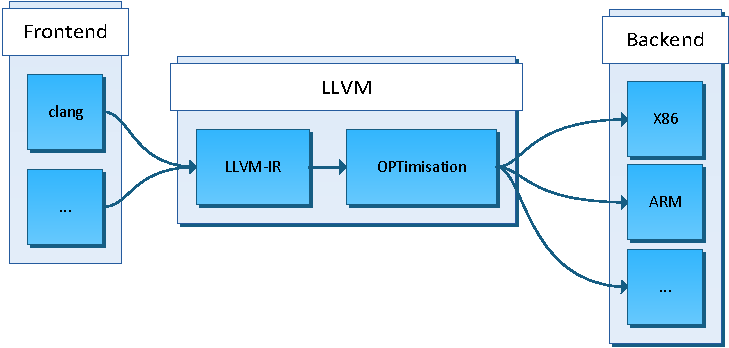
\includegraphics[width=.9\textwidth]{imgs/clang.pdf}
  \end{block}
\end{frame}

\begin{frame}{LLVM IR introduction}
  \begin{block}{Some definitions}
    \begin{itemize}
      \item Kind of structured typed assembly
      \item Module
        \begin{itemize}
          \item Global variables
          \item Functions $\Rightarrow$ Basic blocks $\Rightarrow$ Instructions
        \end{itemize}
      \item Single Static Assignment (SSA)
      \item Can be serialized/deserialized into/from a textual form
    \end{itemize}
  \end{block}

  \pause

  \begin{alertblock}{Remarks}
    \begin{itemize}
      \item C ABI is partially resolved
      \item {\bf Not} a portable virtual machine
      \item Clang generates LLVM IR code according to the target architecture/OS
      \item More on all of that later...
    \end{itemize}
  \end{alertblock}
\end{frame}

\begin{frame}[fragile]
  \frametitle{LLVM IR: examples}
  \begin{lstlisting}[caption=C code,language=c,frame=leftline]
#include <stdint.h>
uint16_t add(uint16_t a, uint16_t b) {
  return a+b;
}
  \end{lstlisting}

  \begin{onlyenv}<1>
  \begin{lstlisting}[caption=LLVM IR for amd64/Linux with -O1,language=llvm,frame=leftline]
$ clang-6.0 -S -emit-llvm -O1 -o - add.c
source_filename = "add.c"
target datalayout = "e-m:e-i64:64-f80:128-n8:16:32:64-S128"
target triple = "x86_64-unknown-linux-gnu"

define zeroext i16 @add(i16 zeroext %a, i16 zeroext %b) {
  %1 = add i16 %b, %a
  ret i16 %1
}
  \end{lstlisting}
  \end{onlyenv}

  \begin{onlyenv}<2>
  \begin{lstlisting}[caption=LLVM IR for amd64/Linux w/o opt,language=llvm,frame=leftline]{Name}
define zeroext i16 @add(i16 zeroext %a, i16 zeroext %b) {
  %1 = alloca i16, align 2
  %2 = alloca i16, align 2
  store i16 %a, i16* %1, align 2
  store i16 %b, i16* %2, align 2
  %3 = load i16, i16* %1, align 2
  %4 = zext i16 %3 to i32
  %5 = load i16, i16* %2, align 2
  %6 = zext i16 %5 to i32
  %7 = add nsw i32 %4, %6
  %8 = trunc i32 %7 to i16
  ret i16 %8
}
  \end{lstlisting}
  \end{onlyenv}
\end{frame}

\begin{frame}[fragile]
  \frametitle{LLVM IR: optimisations}

  \begin{block}{Applying passes one by one}
    \begin{itemize}
      \item {\tt opt} applies a list of pass on the LLVM IR
      \item Useful to debug / understand passes
    \end{itemize}
  \end{block}

  \vspace{-1em}
  \begin{columns}[t]
    \begin{column}{0.5\textwidth}
      \begin{lstlisting}[caption=Non-optimized IR,language=llvm,frame=leftline]
define zeroext i16 @add(i16 zeroext %a, i16 zeroext %b) {
  %1 = alloca i16, align 2
  %2 = alloca i16, align 2
  store i16 %a, i16* %1, align 2
  store i16 %b, i16* %2, align 2
  %3 = load i16, i16* %1, align 2
  %4 = zext i16 %3 to i32
  %5 = load i16, i16* %2, align 2
  %6 = zext i16 %5 to i32
  %7 = add nsw i32 %4, %6
  %8 = trunc i32 %7 to i16
  ret i16 %8
}
      \end{lstlisting}
    \end{column}
    \begin{column}{0.5\textwidth}
      \begin{lstlisting}[caption={\tt opt -mem2reg -S},language=llvm,frame=leftline]
define zeroext i16 @add(i16 zeroext %a, i16 zeroext %b) #0 {
  %1 = zext i16 %a to i32
  %2 = zext i16 %b to i32
  %3 = add nsw i32 %1, %2
  %4 = trunc i32 %3 to i16
  ret i16 %4
}
      \end{lstlisting}
      \vspace{-1em}
      \pause
      \begin{lstlisting}[caption={\tt opt -mem2reg -instcombine -S},language=llvm,frame=leftline]
define zeroext i16 @add(i16 zeroext %a, i16 zeroext %b) #0 {
  %1 = add i16 %a, %b
  ret i16 %1
}
      \end{lstlisting}
    \end{column}
  \end{columns}

\end{frame}

\begin{frame}{LLVM IR: control flow and vectorization}
  \begin{block}{Demo}
    \begin{itemize}
      \item Simple control flow
      \item Loop w/o vectorization
      \item Loop with vectorization
      \item Examples of non-portability
    \end{itemize}
  \end{block}

\end{frame}

\section{Find and "fix" the bug}

\begin{frame}{Minimal reproducer}
  \begin{block}{Find a minimal C++ file with the bug}
    \begin{itemize}
      \item Hints given by {\tt -Rpass-analysis=loop-vectorize}
      \item Start from there and understand what's going on
      \item Other hint: Pythran uses expression templates
    \end{itemize}
  \end{block}

  \begin{block}{Reduced test case}
    \begin{center}
      \url{https://godbolt.org/z/val3Xm}
      %\url{http://localhost:10240/z/Ji5w-L}
    \end{center}
  \end{block}
\end{frame}

\begin{frame}[fragile]{Gathering clues}
  \begin{block}{Diffing LLVM IRs}
    \begin{itemize}
      \item We know the C version is vectorized
      \item Let's compare the two non-vectorized version of the LLVM IR
      \item It might help us understand where something fails
    \end{itemize}
    \begin{center}
      \url{https://godbolt.org/z/VV6S-h}
      %\url{http://localhost:10240/z/6kcVRn}
    \end{center}
  \end{block}

  \pause

  \begin{block}{Have a little talk with the vectorizer (notebook)}
    \begin{lstlisting}
$ clang++-4.0 -O2 -std=c++12 op_zip_iterator.cpp -Rpass-missed=loop-vectorize -Rpass-analysis=loop-vectorize -c -o /dev/null
/usr/include/c++/8/bits/stl_algobase.h:322:4: remark: @@\bfseries loop not vectorized: value that could not be identified as reduction is used outside the loop@ [-Rpass-analysis=loop-vectorize]
          for(_Distance __n = __last - __first; __n > 0; --__n)
    \end{lstlisting}
  \end{block}

\end{frame}

\begin{frame}[fragile]{Checking the LLVM source code}
  \begin{block}{{\tt rgrep 'reduction is used outside the loop' llvm/lib}}
    \begin{lstlisting}[language=c]
// For each block in the loop.
for (BasicBlock *BB : TheLoop->blocks()) {
  // Scan the instructions in the block and look for hazards.
  for (Instruction &I : *BB) {
    if (auto *Phi = dyn_cast<PHINode>(&I)) {
      // [...]
      InductionDescriptor ID;
      if (InductionDescriptor::isInductionPHI(Phi, TheLoop, PSE, ID)) {
        addInductionPhi(Phi, ID, AllowedExit);
        // [...]
        continue;
      }
      // [...]
      // As a last resort, coerce the PHI to a AddRec expression
      // and re-try classifying it a an induction PHI.
      if (InductionDescriptor::isInductionPHI(Phi, TheLoop, PSE, ID, true)) {
        addInductionPhi(Phi, ID, AllowedExit);
        continue;
      }
      @@\bfseries ORE->emit(@createMissedAnalysis("NonReductionValueUsedOutsideLoop", Phi)
                << "value that could not be identified as "
                   "reduction is used outside the loop"@@\bfseries)@;
      @@\bfseries DEBUG(@dbgs() << "LV: Found an unidentified PHI." << *Phi << "\n"@@\bfseries)@;
      return false;
    \end{lstlisting}
  \end{block}
\end{frame}

\begin{frame}{Getting the problematic PHI node}
  \begin{block}{LLVM in debug mode}
    \begin{itemize}
      \item The {\tt DEBUG} macro can give us the PHI node that seems to cause trouble
      \item {\tt DEBUG} macros are deactivated in release builds
      \item We need to compile LLVM in debug mode and print debug informations
    \end{itemize}
  \end{block}

  \pause

  \begin{block}{Compilation}
    \begin{itemize}
      \item Lots of information here: \url{https://llvm.org/docs/CMake.html}
      \item Download LLVM and Clang 4.0 sources from \url{http://releases.llvm.org}, then:
      \item {\tt cmake -DCMAKE\_BUILD\_TYPE=Debug -DBUILD\_SHARED\_LIBS=ON -DLLVM\_OPTIMIZED\_TABLEGEN=ON -G ninja .. \&\& ninja}
      \item Grab a coffee, go for a run, this can take some time depending on your hardware ($\sim$20min on mine)
    \end{itemize}
  \end{block}
\end{frame}

\begin{frame}[fragile]{Getting the problematic PHI node}
  \begin{block}{Show debug informations}
    \begin{lstlisting}
$ /path/to/build/bin/clang++ @@\bfseries -mllvm -debug -mllvm -debug-only=loop-vectorize -Rpass-analysis=vectorize@ -O2  code/op_zip_iterator.cpp -Xclang -discard-value-names -c -o /dev/null  -std=c++11 
LV: Checking a loop in "_Z2opPj16add_zip_iteratorS0_" from /usr/lib/gcc/x86_64-linux-gnu/8/../../../../include/c++/8/bits/stl_algobase.h:322:4
LV: Loop hints: force=? width=0 unroll=0
@@\bfseries LV: Found a loop: for.body.i.i.i.i@
@@\bfseries LV: Found an induction variable.@
@@\bfseries LV: Found an induction variable.@
@@\bfseries LV: Found an induction variable.@
In file included from /home/aguinet/confs/18-10-16-cppfrug-llvm/code/op_zip_iterator.cpp:1:
In file included from /usr/lib/gcc/x86_64-linux-gnu/8/../../../../include/c++/8/algorithm:61:
/usr/lib/gcc/x86_64-linux-gnu/8/../../../../include/c++/8/bits/stl_algobase.h:322:4: remark: loop not vectorized: value that could not be identified as reduction is used outside the loop
      [-Rpass-analysis=loop-vectorize]
          for(_Distance __n = __last - __first; __n > 0; --__n)
          ^
@@\bfseries LV: Found an unidentified PHI.  \%16 = phi i64 [ \%22, \%12 ], [ \%6, \%10 ]@
LV: Can't vectorize the instructions or CFG
LV: Not vectorizing: Cannot prove legality.
    \end{lstlisting}
  \end{block}
\end{frame}

\begin{frame}[fragile,t]{Putting the pieces together}
  \vspace{-1em}
  \begin{columns}[t]
    \begin{column}{.6\textwidth}
      \begin{lstlisting}[language=llvm,basicstyle=\tiny\ttfamily,identifierstyle=\tiny\ttfamily]
define void @op_distance(i32* %res, i32* %it.a, i32* %it.b, i32* %it_end.a, i32* %it_end.b) {
  %it.a_int = ptrtoint i32* %it.a to i64
  %it_end.a_int = ptrtoint i32* %it_end.a to i64
  %8 = sub i64 %it.a_int, %it_end.a_int
  %9 = icmp sgt i64 %8, 0
  br i1 %9, label %loop_header, label %ret

; <label>:loop_header:                              ; preds = %loop, %entry
  %count = lshr exact i64 %8, 2
  br label %loop

; <label>:loop:                                     ; preds = %loop, %loop_header
  %cur_count = phi i64 [ %next_count, %loop ], [ %count, %loop_header ]
  %cur_res = phi i32* [ %next_res, %loop ], [ %res, %loop_header ]
  %cur_it.b = phi i32* [ %next_it.b, %loop ], [ %it.b, %loop_header ]
  @@\bfseries \%cur\_it.a\_int = phi i64 [ \%next\_it.a\_int, \%loop ], [ \%it.a\_int, \%loop\_header ]@
  @@\bfseries \%17 = inttoptr i64 \%16 to i32*@
  %18 = load i32, i32* %17, align 4, !tbaa !1
  %19 = load i32, i32* %15, align 4, !tbaa !1
  %20 = add i32 %19, %18
  store i32 %20, i32* %14, align 4, !tbaa !1
  %21 = getelementptr inbounds i32, i32* %17, i64 1
  @@\bfseries \%next\_it.a\_int = ptrtoint i32* \%21 to i64@
  @@\bfseries \%next\_it.b = getelementptr inbounds i32, i32* \%15, i64 1@
  %next_res = getelementptr inbounds i32, i32* %14, i64 1
  %next_count = add nsw i64 %cur_count, -1
  %26 = icmp sgt i64 %cur_count, 1
  br i1 %26, label %loop, label %loop_end
; <label>:loop_end:                                     ; preds = %loop
  br label %ret

; <label>:ret:                                     ; preds = %loop_end, %entry
  ret void
}
      \end{lstlisting}
    \end{column}
    \begin{column}{.4\textwidth}
      \begin{small}
      \begin{block}{What's happening here?}
        \begin{itemize}
          \item The loop vectorizer checks that everything in the loop can be vectorized
          \item It relies on an analysis that finds induction variables
          \item PHI node {\tt \%cur\_it.a\_int} isn't considered as one (and should be)
          \item Because of the {\tt inttoptr <=> ptrtoint} round-trip?
        \end{itemize}
      \end{block}
      \end{small}
    \end{column}
  \end{columns}
\end{frame}

\begin{frame}[fragile]{Further analyses}
  \begin{block}{The "Scalar evolution" analysis in LLVM}
    \begin{itemize}
      \item In one sentence: "Change in the Value of Scalar Variables Over Iterations of the Loop"
      \item Sentence from this nice talk about it in EuroLLVM 2018: \url{https://www.youtube.com/watch?v=AmjliNp0_00}
      \item Used by the "is an induction variable?" analysis
    \end{itemize}
  \end{block}

  \pause

  \begin{alertblock}{In its source code}
    \begin{lstlisting}[language=c]
// It's tempting to handle inttoptr and ptrtoint as no-ops, however this can
// lead to pointer expressions which cannot safely be expanded to GEPs,
// because ScalarEvolution doesn't respect the GEP aliasing rules when
// simplifying integer expressions.
    \end{lstlisting}

    \begin{itemize}
      \item Looks like these {\tt inttoptr <=> ptrtoint} conversions are the problem!
    \end{itemize}
  \end{alertblock}
\end{frame}

\begin{frame}{One "fix"}
  \begin{block}{Remove the {\tt inttoptr <=> ptrtoint} round-trip}
    \begin{itemize}
      \item Out-of-tree pass that does this: \url{https://github.com/aguinet/llvm-intptrcleanup}
      \item Not sure this is semantically valid, but it will show that our theories are valid
    \end{itemize}
  \end{block}

  \pause

  \begin{alertblock}{Result}
    \begin{itemize}
      \item Pass is registered before vectorization (in the pipeline)
      \item {\tt inttoptr <=> ptrtoint} round-trips are removed
      \item Vectorisation happens!
    \end{itemize}
    \begin{center}
      \url{http://localhost:10240/z/aWxbpR}
    \end{center}
  \end{alertblock}
\end{frame}

\begin{frame}[fragile]{Going further}
  \begin{block}{Which pass creates this?}
    \begin{itemize}
      \item Using clang in debug mode, we see
        \begin{lstlisting}[language=llvm]
__first.sroa.0.012.i.i.i.i = phi i64 [%5, %for.body.i.i.i.i], [%0, %for.body.preheader.i.i.i.i]
        \end{lstlisting}
      \item SROA = Scalar Replacement of Aggregates
    \end{itemize}
  \end{block}

  \begin{block}{Scalar Replacement of Aggregates}
    \begin{itemize}
      \item "This transform breaks up alloca instructions of aggregate type
        (structure or array) into individual alloca instructions for each
        member if possible. Then, if possible, it transforms the individual
        alloca instructions into nice clean scalar SSA form."
        \footnote{\url{https://llvm.org/docs/Passes.html\#sroa-scalar-replacement-of-aggregates}}
    \end{itemize}
  \end{block}

  \begin{block}{The proper fix}
    \begin{itemize}
      \item Properly fixing probably means fixing SROA
    \end{itemize}
  \end{block}
\end{frame}

\begin{frame}{Reporting the bug}
  \begin{block}{Bug reporting}
    \begin{itemize}
      \item LLVM bug tracker: \url{https://bugs.llvm.org/}. Registration is
        closed, an email needs to be sent to get an account.
      \item {\tt llvm-dev} mailing list: to ask for help on how to really fix
        the issue. People are generally reactive!
    \end{itemize}
  \end{block}

  \begin{alertblock}{Related links}
    \begin{itemize}
      \item Bug tracker: \url{https://bugs.llvm.org/show_bug.cgi?id=33532}
      \item Mailing-list: \url{http://lists.llvm.org/pipermail/llvm-dev/2017-June/114300.html}
    \end{itemize}
  \end{alertblock}

\end{frame}

\section{Conclusion \& discussion}

\begin{frame}{Conclusion}
  \begin{block}{Did we fix the Pythran code vectorization?}
    \begin{itemize}
      \item Let's try it...
      \pause
      \item ...somehow we fixed our test case, but not the whole Pythran case
      \item clang 7 still fails at this!
      \item So we need to re-do this again :)
    \end{itemize}
  \end{block}

  \pause

  \begin{alertblock}{What did we learn? (I hope)}
    \begin{itemize}
      \item Compilers have lots of ways to debug their analyses
      \item How to dig into them to understand what's happening
      \item Compiling communities are receptives to this kind of issues
    \end{itemize}
  \end{alertblock}
\end{frame}

\begin{frame}{Discussion}
  \begin{block}{Zero-cost abstractions?}
    \begin{itemize}
      \item Zero-cost abstractions are often presented as an advantage of C++
      \item But {\bf nothing guarantees} it in the {\bf standard} 
      \item It works because we have good {\bf optimising compilers}!
    \end{itemize}
  \end{block}

  \pause

  \begin{alertblock}{Issue}
    \begin{center}
      When performance is a user contract, there's no way {\bf standard} way to
      guarantee many of it!
    \end{center}
  \end{alertblock}
\end{frame}

\begin{frame}{Guaranteed optimisations}
  \begin{block}{Guaranteed optimisations?}
    \begin{itemize}
      \item {\tt pragma}s to trigger an error if an optimisation fails?
      \item User-driver optimisation flow?
      \item Level of optimisations guaranteed by the C++ standard?
    \end{itemize}
  \end{block}

  \pause
  \begin{alertblock}{Ideas}
    \begin{itemize}
      \item Use {\tt FileCheck}
        \begin{itemize}
          \item Check the generated assembly (problem: this is platform-dependant)
          \item Check the generated LLVM IR (still platform-dependant, but more generic)
          \item Demo!
        \end{itemize}
      \item C backend for the LLVM IR for an easier-to-read representation?
    \end{itemize}
  \end{alertblock}
\end{frame}
% pragmas to drive optimisations?
% pragmas to have an error if an optimisation fails?
  % FileCheck to check final assembly
% C backend for the LLVM IR aimed at visualising the final code? (not
% necessarly recompile it)
% standard optimisations?

\section{Bonus}

\begin{frame}[fragile]
  \frametitle{How does this compile? (Linux/x86-64)}

  \begin{block}{XOR two buffer of 16 bytes}
    \begin{lstlisting}[language=c]
void xorBlocks(uint8_t* Out, uint8_t const* In) {
  for (size_t I = 0; I < 16; ++I) {
    Out[I] ^= In[I];
  }
}
    \end{lstlisting}
  \end{block}

  \begin{center}
    \url{https://godbolt.org/z/MpmttL}
    %\url{http://localhost:10240/z/MpmttL}
  \end{center}
\end{frame}

\begin{frame}{Questions?}
  \begin{block}{Thanks for your attention!}
    \vspace{1em}
    \begin{center}
      Questions?
    \end{center}
    \vspace{.5em}
  \end{block}

  \begin{block}{Acknowledgment}
    Serge Guelton for the Pythran project and the discussions regarding this talk!
  \end{block}

  \begin{block}{Contact}
    \begin{center}
      \begin{tabular}{ll}
        \mail & \href{mailto:adrien@guinet.me}{adrien@guinet.me}\\
        \github & \href{https://github.com/aguinet}{https://github.com/aguinet}\\
        \twitter & \href{https://twitter.com/adriengnt}{adriengnt}\\
      \end{tabular}
    \end{center}
  \end{block}
\end{frame}
%\bgroup
%%\usebackgroundtemplate{\includegraphics[width=\paperwidth,height=\paperheight]{logo/qb-card.pdf}}
%\begin{frame}[plain]
%    \begin{center}
%      Questions?
%    \end{center}
%    \vfill
%\end{frame}
%%\egroup


\end{document}
